\clearpage
\newpage
\section{Results}
\subsection{Limits}
\label{sec:stats}
We set limits on the production cross-section of 
the $\wpr_R$ boson. We compare the number 
of observed events to the number of events expected given the new physics model. We use the following formula:
\begin{eqnarray}
N_{\textrm{expected}} = \sigma_{\wpr_R} \times B_{\wpr_R \rightarrow tb;W \to hadrons} \times \varepsilon \times \emph{L}
\end{eqnarray}
where $\sigma_{\wpr_R}$ is the $\wpr_R$ cross-section, $B_{\wpr_R \rightarrow \tbbar;W \to hadrons}$ is the branching ratio 
$\wpr_R \to \tbbar$ with the W decay constrained to the hadronic branching fraction, $\varepsilon$ is the signal efficiency corrected by data-driven scale factors and $\emph{L}$ is the integrated luminosity of our dataset. 

We perform a shape analysis using the $\mathrm{M_{tb}}$ distribution.  We use a binned likelihood fit to compare the distribution from the $\wpr$ boson signal 
hypothesis with the Standard Model distribution produced by our background estimation procedure.  

\label{sec:Theta}
To set shape based limits, the Theta package \cite{theta} is used.  We use a Bayesian method to extract 95\% CL upper limits 
on the production of a right-handed $\wpr$ particle.  

A Poisson model is used in each bin of our analysis.  For each bin, the mean of the Poisson distribution is:
\begin{eqnarray}
\mu_i = \sum_k \beta_k \times T_{k,i}
\end{eqnarray}
here, k includes the signal and background models, and T represents the fraction of events expected for each process $k$ in bin $i$.

The likelihood function is then:
\begin{eqnarray}
L(\beta_k) = \prod^{N_{bins}}_i \frac{\mu_i \times e^{-\mu_i}}{N^{data}_i!}
\end{eqnarray}
Where $\mu_i$ is the mean of the Poisson distribution in bin $i$, given in terms of $T$, the number of events expected from the process $k$.

The Theta package performs pseudoexperiments to calculate 68\% and 95\% upper bounds on the limit bands.  
The pseudoexperiments take into account systematic effects as nuisance parameters.  These nuisance parameters 
are varied within their uncertainties and the posterior is refitted for each pseudoexperiment.  

The uncertainty in the jet energy scale, $Q^2$ scale, $\pt$ re-weighting, trigger, $SF_b$, QCD background uncertainties, and jet energy resolution are taken 
as shape based uncertainties, and the other sources of uncertainty are taken as overall normalizations.  

The limits from Theta are shown in Figure \ref{figs:thetalimit}.

\begin{table}
\begin{center}
\bf{Cross-Section Upper Limits}\\
\begin{tabular}{c||c|c|c|c}
\hline
\hline
\bf{$\mathrm{M_{\tbbar}}$} & \bf{observed}  & \bf{expected} & \bf{expected 1$\sigma$}  & \bf{expected 2$\sigma$} \\
\hline
\hline
1300 & 0.146 & 0.117 & 0.080,0.166 & 0.057,0.229\\
\hline
1500 & 0.059 & 0.078 & 0.056,0.112 & 0.040,0.163\\
\hline
1700 & 0.050 & 0.066 & 0.047,0.097 & 0.034,0.130\\
\hline
1900 & 0.055 & 0.062 & 0.043,0.091 & 0.032,0.126\\
\hline
2100 & 0.064 & 0.064 & 0.046,0.093 & 0.036,0.140\\
\hline
2300 & 0.073 & 0.069 & 0.052,0.098 & 0.042,0.147\\
\hline
2700 & 0.093 & 0.106 & 0.082,0.146 & 0.071,0.211\\
\hline
\end{tabular}
\end{center}
\caption{$\wpr_R$ cross-section upper limits for given $\mathrm{M_{\tbbar}}$ values.  Cross-section is in units of pb.}
\label{table:upperxsec}
\end{table}


\begin{figure}[htcb]
\centering
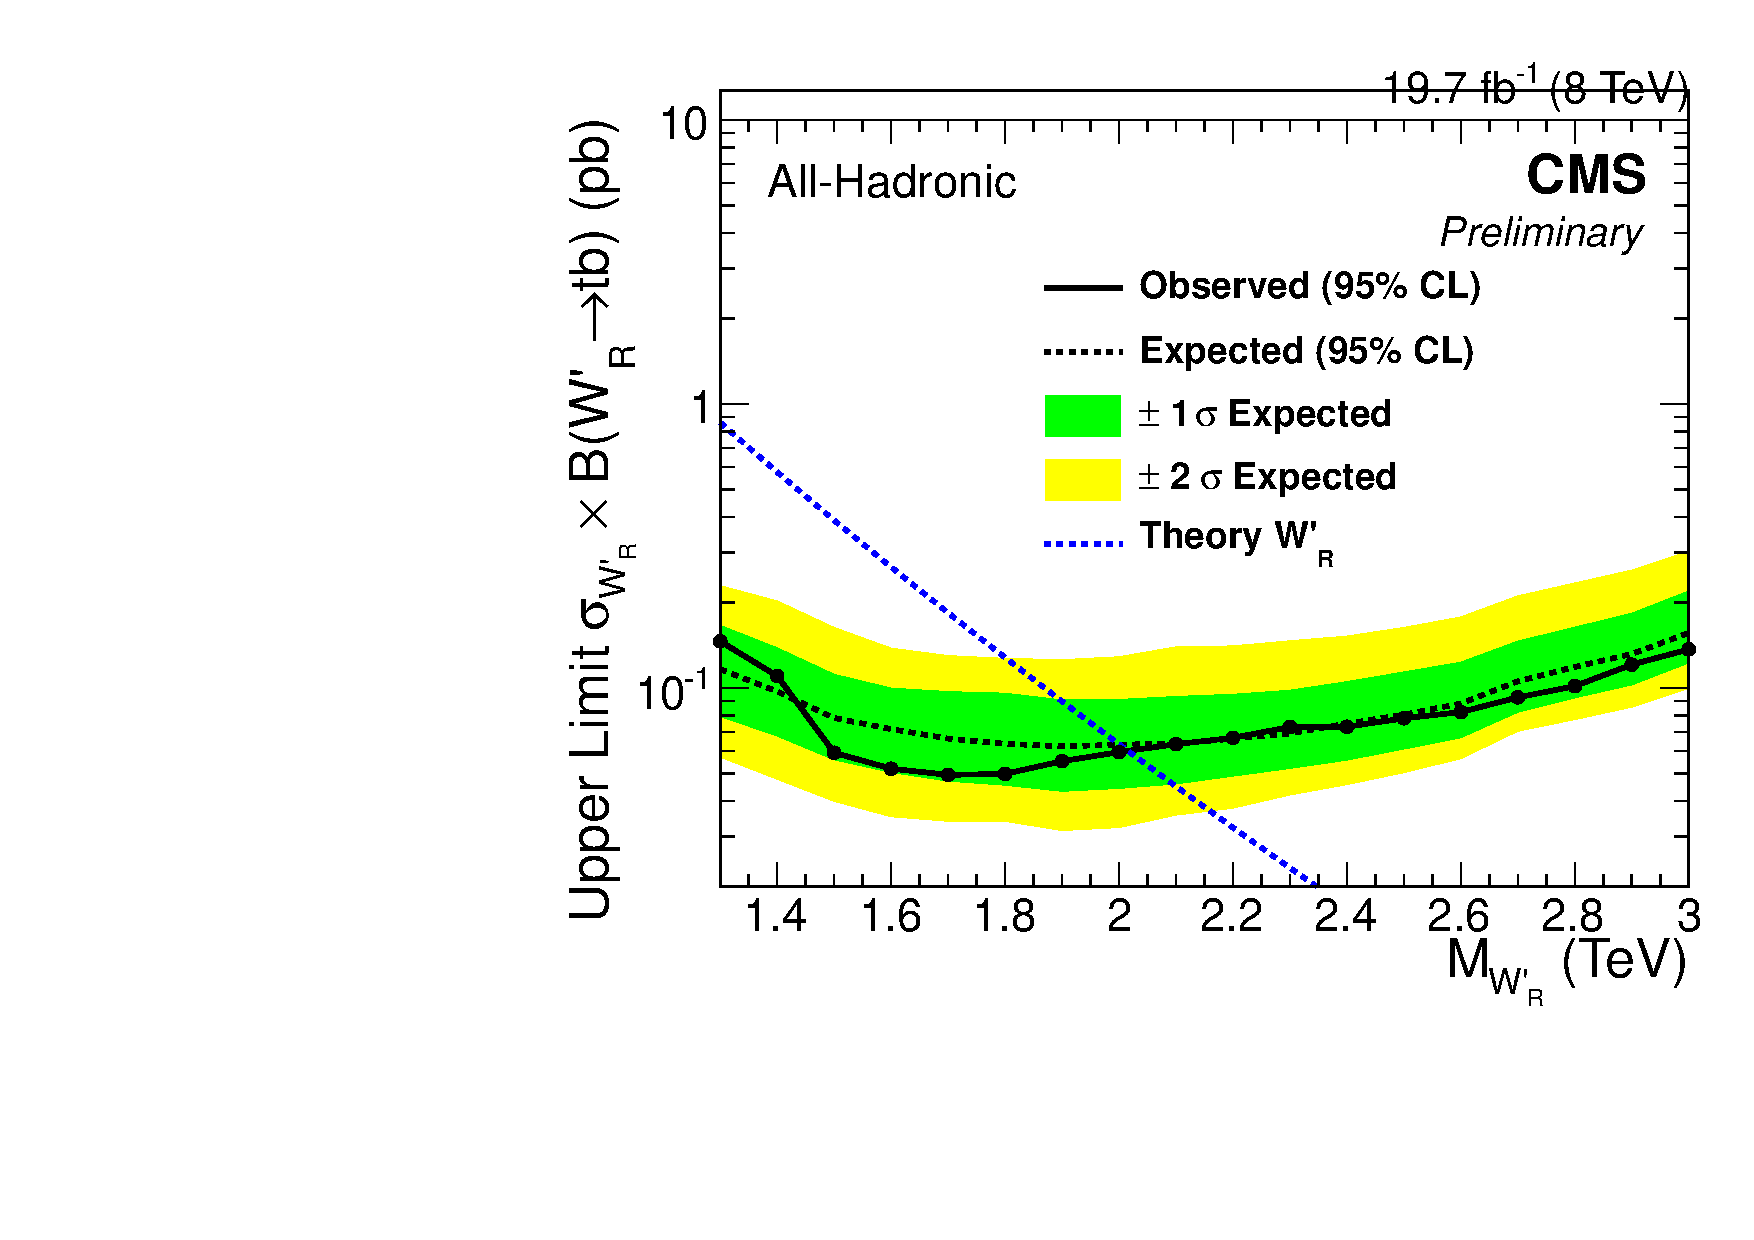
\includegraphics[width=1.0\textwidth]{AN-13-004/figs/limits_theta_Hadroniccomb_log.pdf}
\caption{The $\wpr_{R}$ boson 95\% C.L. production cross-section limits.  The expected (black) and observed (red) limits as well as $\wpr_{R}$ boson theoretical cross-section (blue) are plotted for comparison.  
The uncertainty in the expected limit band is shown in light ($\pm$1$\sigma$) and dark grey ($\pm$2$\sigma$).
These limits were extracted using the Theta limit setting framework.}
\label{figs:thetalimit}
\end{figure}



%\begin{figure}[htcb]
%\centering
%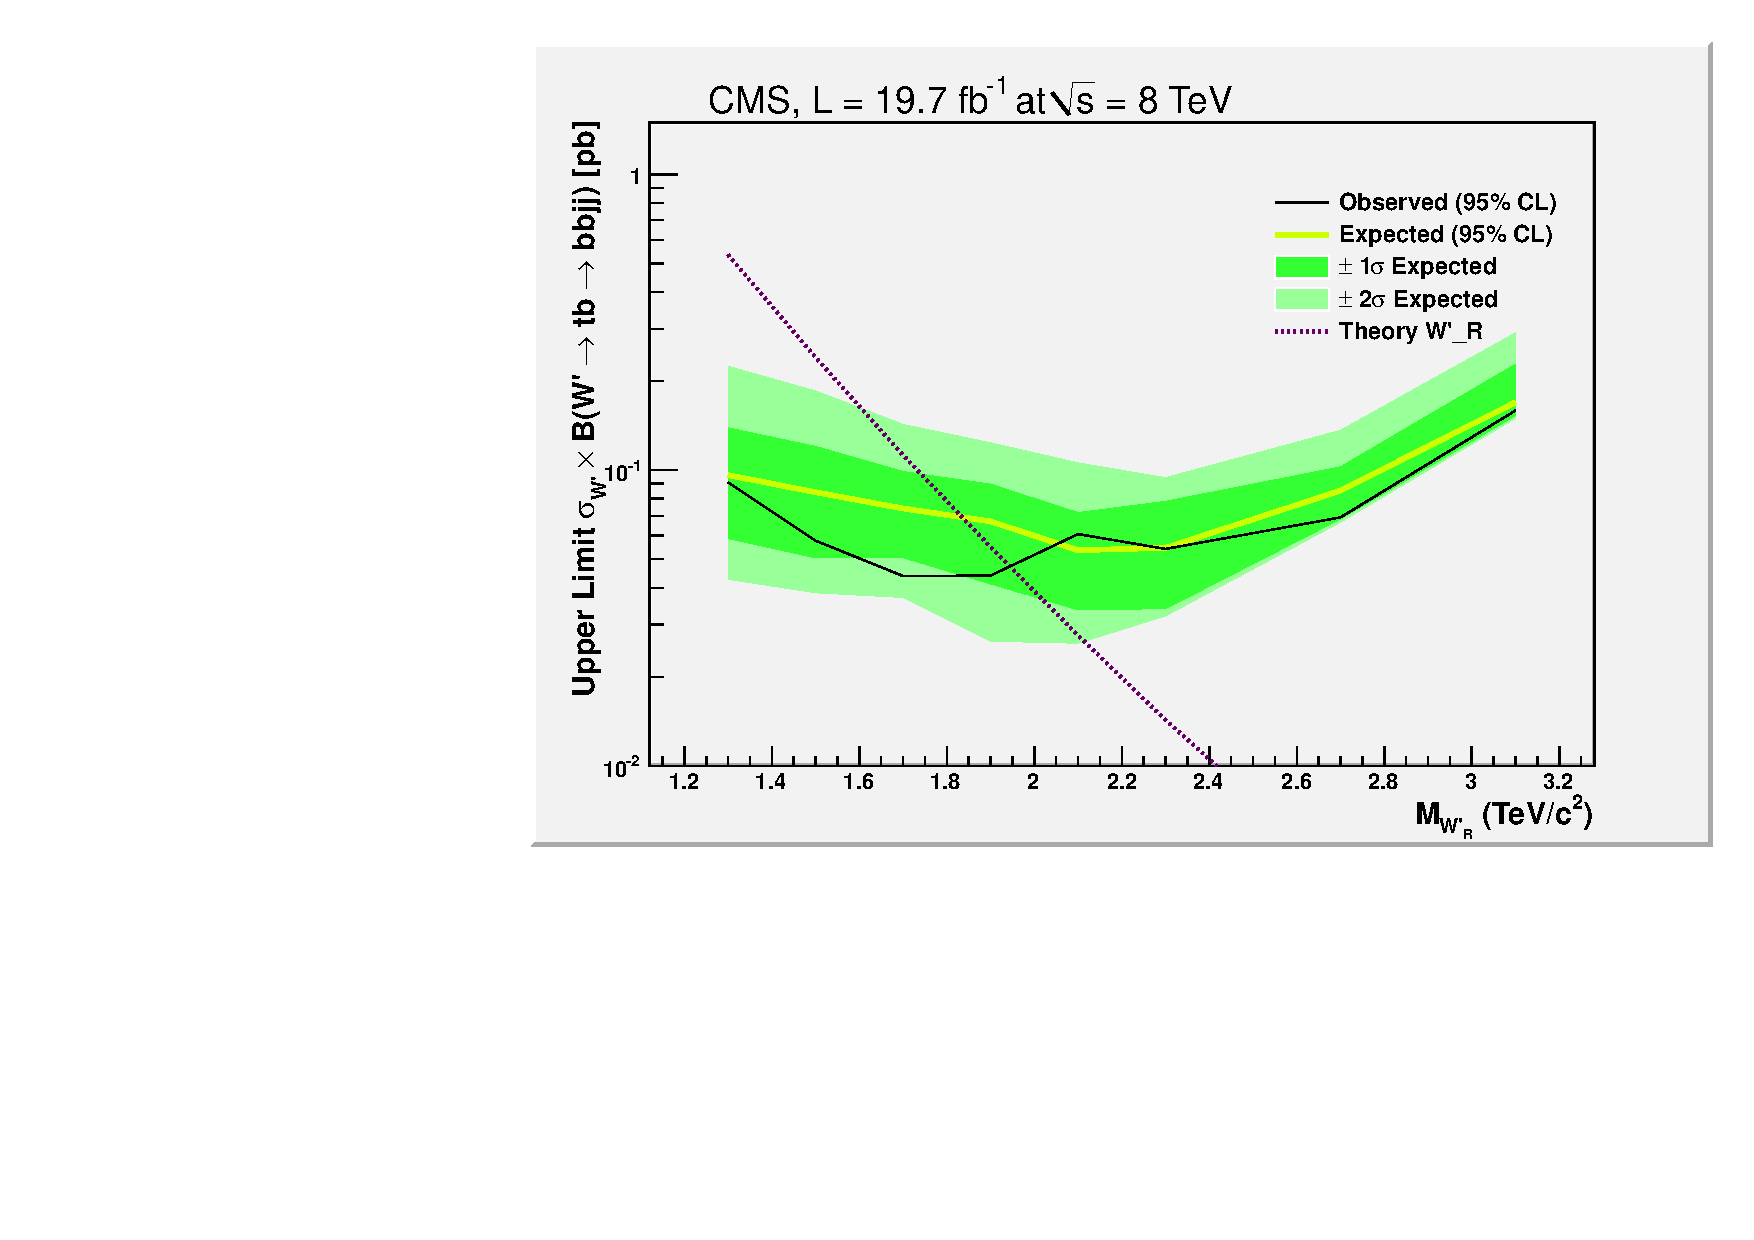
\includegraphics[width=1.0\textwidth]{AN-13-004/figs/forkevin_Jan_.pdf}
%\caption{Cross check of the Theta shape-based limits (Figure \ref{figs:thetalimit}) using the Higgs Combine tool.  The limits are extracted using a simple counting experiment.}
%\label{figs:limit}
%\end{figure}


\begin{sidewaystable}
\begin{center}
\bf{Nuisance Parameters}\\
\scalebox{0.5}{
\begin{tabular}{c||c|c|c|c|c|c|c|c|c|c|c}
\hline\hline
\bf{Sample} & \bf{JER} & \bf{JES} & \bf{QCD total} & \bf{b-tagging}  & \bf{$Q^2$}  & \bf{Trigger} & \bf{CA btag SF} & \bf{$\pt$ Re-weight}  & \bf{Lumi} & \bf{$\ttbar$ Norm} & \bf{Subjet SF}  \\
\hline\hline
wp1300 & 0.031 $\pm$ 1.186 & -0.722 $\pm$ 0.855 & -0.486 $\pm$ 0.657 & -0.030 $\pm$ 1.014 & -0.278 $\pm$ 1.337 & 0.002 $\pm$ 1.000 & 0.000 $\pm$ 1.006 & 0.183 $\pm$ 0.649 & 0.000 $\pm$ 1.000 & 0.105 $\pm$ 1.007 & 0.000 $\pm$ 1.001\\
wp1500 & 0.067 $\pm$ 1.111 & -0.905 $\pm$ 0.370 & -0.483 $\pm$ 0.532 & 0.197 $\pm$ 0.884 & 0.420 $\pm$ 0.840 & 0.006 $\pm$ 1.969 & 0.119 $\pm$ 1.683 & -0.133 $\pm$ 0.481 & 0.155 $\pm$ 1.428 & 0.116 $\pm$ 0.901 & -0.116 $\pm$ 0.934\\
wp1700 & 0.094 $\pm$ 1.168 & -0.727 $\pm$ 0.556 & -0.381 $\pm$ 0.523 & 0.058 $\pm$ 0.950 & 0.482 $\pm$ 1.097 & 0.070 $\pm$ 1.045 & 0.013 $\pm$ 1.700 & -0.051 $\pm$ 0.520 & 0.017 $\pm$ 1.462 & 0.173 $\pm$ 0.911 & 0.093 $\pm$ 0.971\\
wp1900 & 0.137 $\pm$ 1.795 & -0.501 $\pm$ 0.302 & -0.340 $\pm$ 0.540 & -0.013 $\pm$ 1.039 & 0.128 $\pm$ 0.285 & -0.004 $\pm$ 1.999 & 0.020 $\pm$ 1.981 & -0.043 $\pm$ 0.473 & 0.026 $\pm$ 1.968 & 0.109 $\pm$ 0.895 & 0.118 $\pm$ 1.136\\
wp2100 & 0.086 $\pm$ 1.333 & -0.617 $\pm$ 0.745 & -0.468 $\pm$ 0.524 & -0.011 $\pm$ 0.999 & 0.511 $\pm$ 0.947 & 0.000 $\pm$ 1.997 & -0.002 $\pm$ 1.981 & 0.030 $\pm$ 0.514 & -0.003 $\pm$ 1.967 & 0.125 $\pm$ 0.905 & -0.013 $\pm$ 1.129\\
wp2300 & 0.074 $\pm$ 1.079 & -0.685 $\pm$ 0.780 & -0.500 $\pm$ 0.714 & -0.016 $\pm$ 1.015 & 0.477 $\pm$ 0.714 & 0.000 $\pm$ 1.002 & 0.000 $\pm$ 1.980 & -0.001 $\pm$ 0.561 & 0.000 $\pm$ 1.964 & 0.131 $\pm$ 0.939 & 0.000 $\pm$ 1.090\\
wp2700 & 0.259 $\pm$ 1.349 & -0.643 $\pm$ 1.077 & -0.396 $\pm$ 0.550 & -0.054 $\pm$ 1.144 & 0.316 $\pm$ 0.824 & -0.004 $\pm$ 1.997 & 0.000 $\pm$ 1.994 & -0.029 $\pm$ 0.476 & 0.000 $\pm$ 1.991 & 0.103 $\pm$ 0.894 & 0.001 $\pm$ 1.793\\
\hline

\end{tabular}
}
\end{center}
\caption{Nuisance parameters after the fit.  This the nominal value found for the nuisance parameter after the fit in units of input sigma.The numbers listed under sample specify $\wpr_R$ signal MC mass.}
\label{table:nuisance}
\end{sidewaystable}


%\subsection{Crosscheck with Counting Experiment}
%\label{sec:countingexperiment}
%As a sanity check to the shape results, we also perform a simple cut and count experiment for 
%each $\wpr_R$ mass point. The resulting limits are consistent with the limits presented in the previous Section.

%We first pick out, by hand, the peak of the signal distribution and designate a window around it (these windows are documented in table \ref{table:countingtable}). We now apply 
%the same Bayesian technique we used to find shape based limits, but apply it to the entire mass window rather than bin by bin. 

%The counting experiment limits are shown for each mass points in Figure \ref{figs:limit}. Nuisance 
%parameters previously treated as shapes are now integrated and used a simple normalization: the error from an effect is 
%treated as the average change in number of events divided by the total events in that process.  


%\begin{table}
%\begin{center}
%\bf{Counting Experiment Windows}\\
%\begin{tabular}{|c||c|c|}
%\hline
%\bf{$\mathrm{M_{\tbbar}}$} & \bf{Lower}  & \bf{Upper} \\
%\hline
%1300 & 1150 & 1350\\
%\hline
%1500 & 1250 & 1550\\
%\hline
%1700 & 1350 & 1750\\
%\hline
%1900 & 1550 & 1950\\
%\hline
%2100 & 1700 & 2150\\
%\hline
%2300 & 1850 & 2350\\
%\hline
%2700 & 2200 & 2750\\
%\hline
%3100 & 2500 & 3200\\
%\hline
%\end{tabular}
%\end{center}
%\caption{windows used for the counting experiment }
%\label{table:countingtable}
%\end{table}


\subsection{Generalized Coupling Limits}
\label{sec:GCTheta}
To set limits on generic couplings, we use the procedure outlined in \cite{CMS-PAS-B2G-12-010}.  
The full selection for the left-handed and mixed-coupling samples (described in section \ref{sec:datasampleAndSelection}) can be seen in Figure \ref{figs:GCFS}.
For limit setting, we weight our templates (single top, $\wpr_R$, $\wpr_L$, $\wpr_{LR}$) using the following cross-sections respectively:
\begin{eqnarray}\label{eq:xsec}
{\sigma}_{SM} &=& {\sigma}_{\text{singletop}}\\\nonumber
{\sigma}_{R} &=& \left(\left(a^L_{ud} a^L_{tb}\right)^2 + \left(a^R_{ud} a^R_{tb}\right)^2 - \frac{1}{2}\left(\left(a^L_{ud} a^R_{tb}\right)^2 + \left(a^R_{ud} a^L_{tb}\right)^2\right) - a^L_{ud} a^L_{tb}\right){\sigma}_{\wpr_R}\\\nonumber
{\sigma}_{L} &=& \left(a^L_{ud} a^L_{tb}-\frac{1}{2}\left(\left(a^L_{ud} a^R_{tb}\right)^2 +\left(a^R_{ud} a^L_{tb}\right)^2\right)\right){\sigma}_{\wpr_L}\\\nonumber
{\sigma}_{LR} &=& \frac{1}{2}\left(\left(a^L_{ud} a^R_{tb}\right)^2 +\left(a^R_{ud} a^L_{tb}\right)^2\right){\sigma}_{\wpr_{LR}}\\\nonumber
\end{eqnarray}

%The cross-section for single top production for both SM and BSM given the couplings under investigation is given by

%\begin{eqnarray}\label{eq:xsec}
%{\sigma} &=& {\sigma}_{SM} + a^L_{ud}a^L_{tb}
%\left({\sigma}_L - {\sigma}_R - {\sigma}_{SM} \right)  \\ \nonumber
%         &+& \left(\left(a^L_{ud} a^L_{tb}\right)^2 
%          +        \left(a^R_{ud} a^R_{tb}\right)^2\right) {\sigma}_R \\ 
%         &+& \frac{1}{2}\left(\left(a^L_{ud} a^R_{tb}\right)^2 
%          +                   \left(a^R_{ud} a^L_{tb}\right)^2\right)
%\left( {\sigma}_{LR} - {\sigma}_L - {\sigma}_R  \right). 
%\nonumber
%\end{eqnarray}

Where $\sigma_{\wpr_{ij}}$ refers to the cross-section for right, left or mixed-coupling samples and $\sigma_{single top}$ is the 
standard model s-channel single top cross-section.
We assume $a_{ud} = a_{tb}$.  The templates are then summed and limits can be set 
using the resultant yield as the signal process for the given values of $a^L$ and $a^R$.
Because the left-handed and mixed-coupling samples cannot be separated from SM single top, we set limits on the couplings $a^L$ and $a^R$.
The Theta package is used for this computation and limits are calculated using combinations of the couplings from 0 to 1 in increments of 0.1.  Using these limits, we find where 
$M_{\wpr}$ cross-section limits align with theory prediction and plot these values in the $a^L$ and $a^R$ plane.  These points are where we can exclude the $a^L$ and $a^R$ coupling combinations 
for the standard model plus $\wpr$ hypothesis at the given $\wpr$ mass.  The results are shown in Figure \ref{figs:GCLim}.  For this procedure, no systematic uncertainty is considered for the single top contribution 
due to the fact that statistical uncertainty dominates in these templates (see Figure \ref{figs:ST}).  


%There is a known discrepancy in the generalized coupling samples that is apparent after 
%comparing the summed $\wpr_{R}$ and $\wpr_{L}$ $\mathrm{M_{tb}}$ spectrum to this spectrum in $\wpr_{LR}$.  
%These distributions should be identical, but show shape and normalization discrepancies.  
%The normalization effect is between 1\% and 12\% at the 1700$\GeV$ and 2700$\GeV$ mass points respectively.  The comparison can be seen in figure \ref{figs:Gencomp1}.

\begin{figure}[htcb]
\begin{center}
\subfigure{\label{figs:GC1}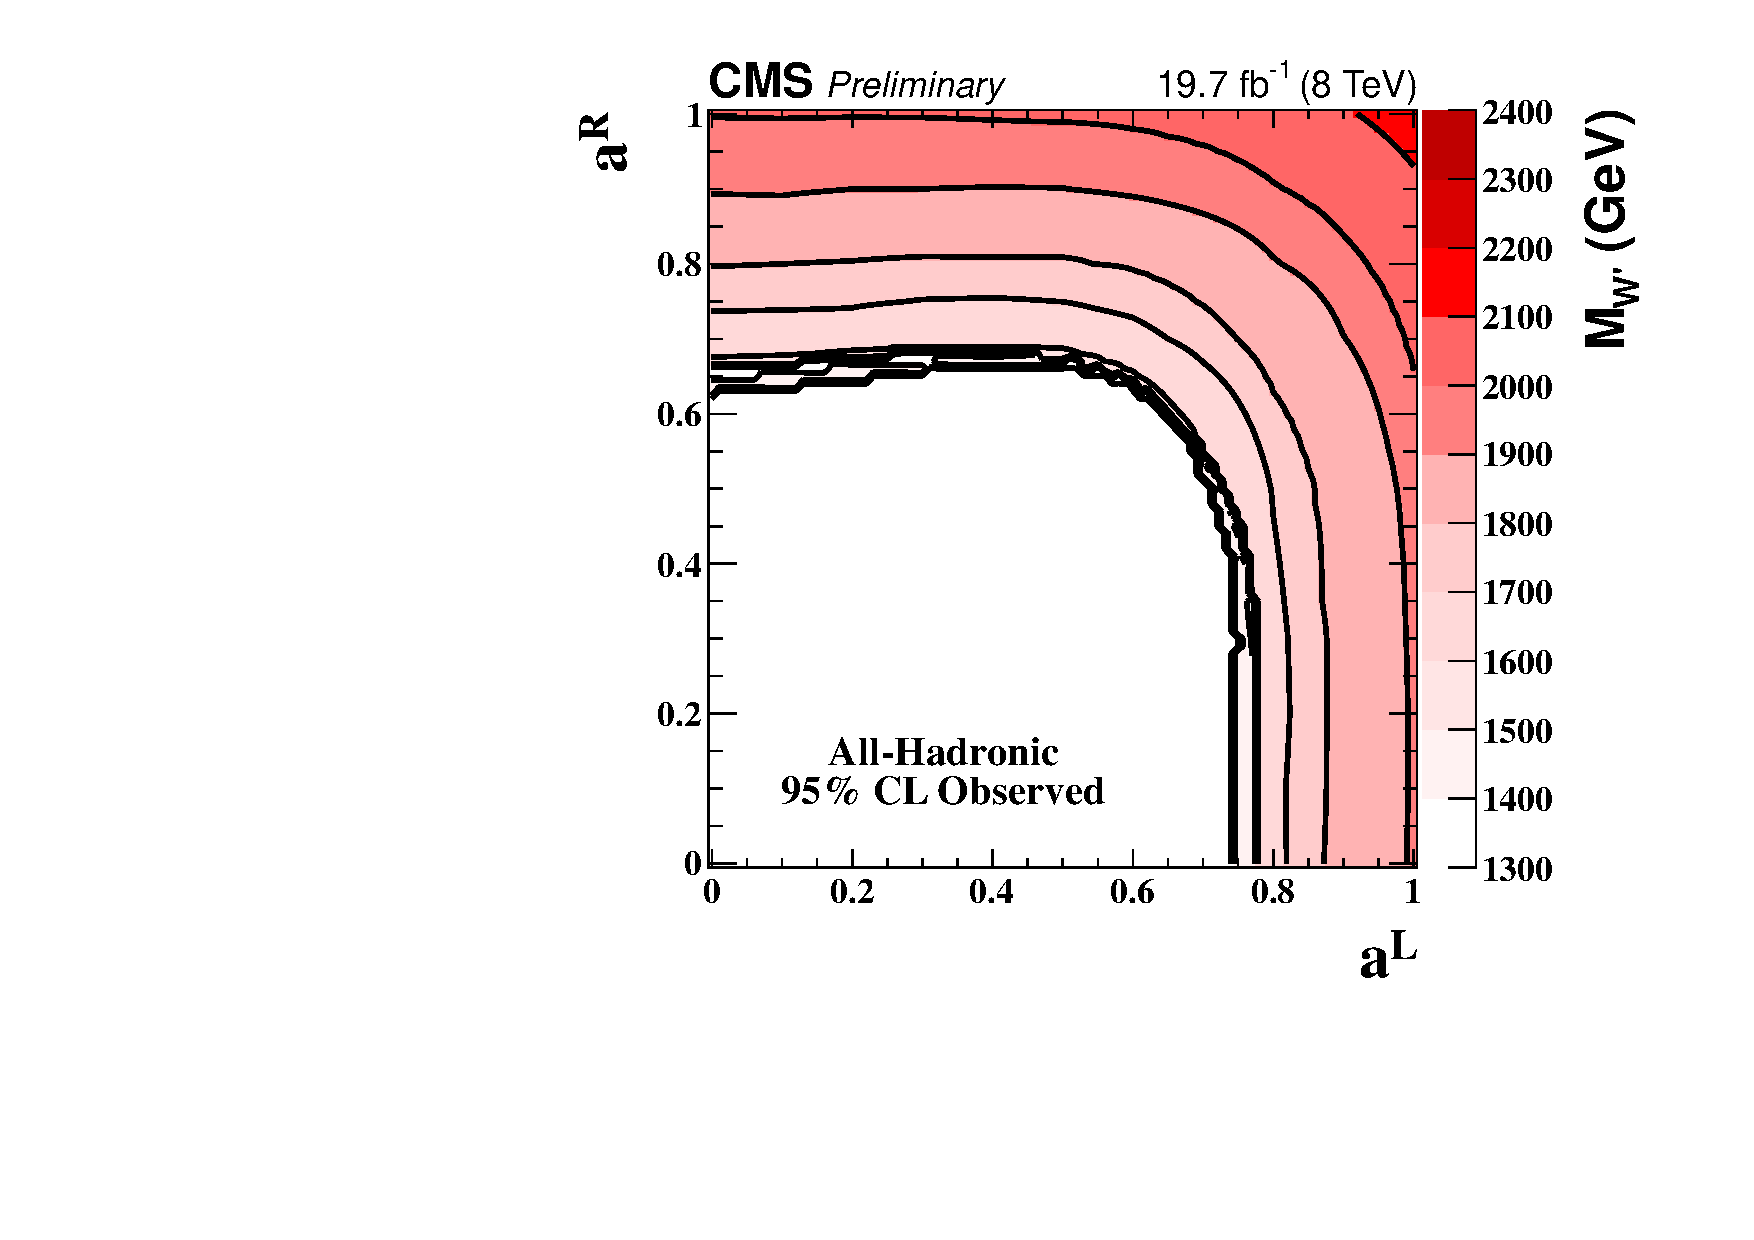
\includegraphics[width=0.7\textwidth]{AN-13-004/figs/contour_Hadronic_observed.pdf}}\\
\subfigure{\label{figs:GC2}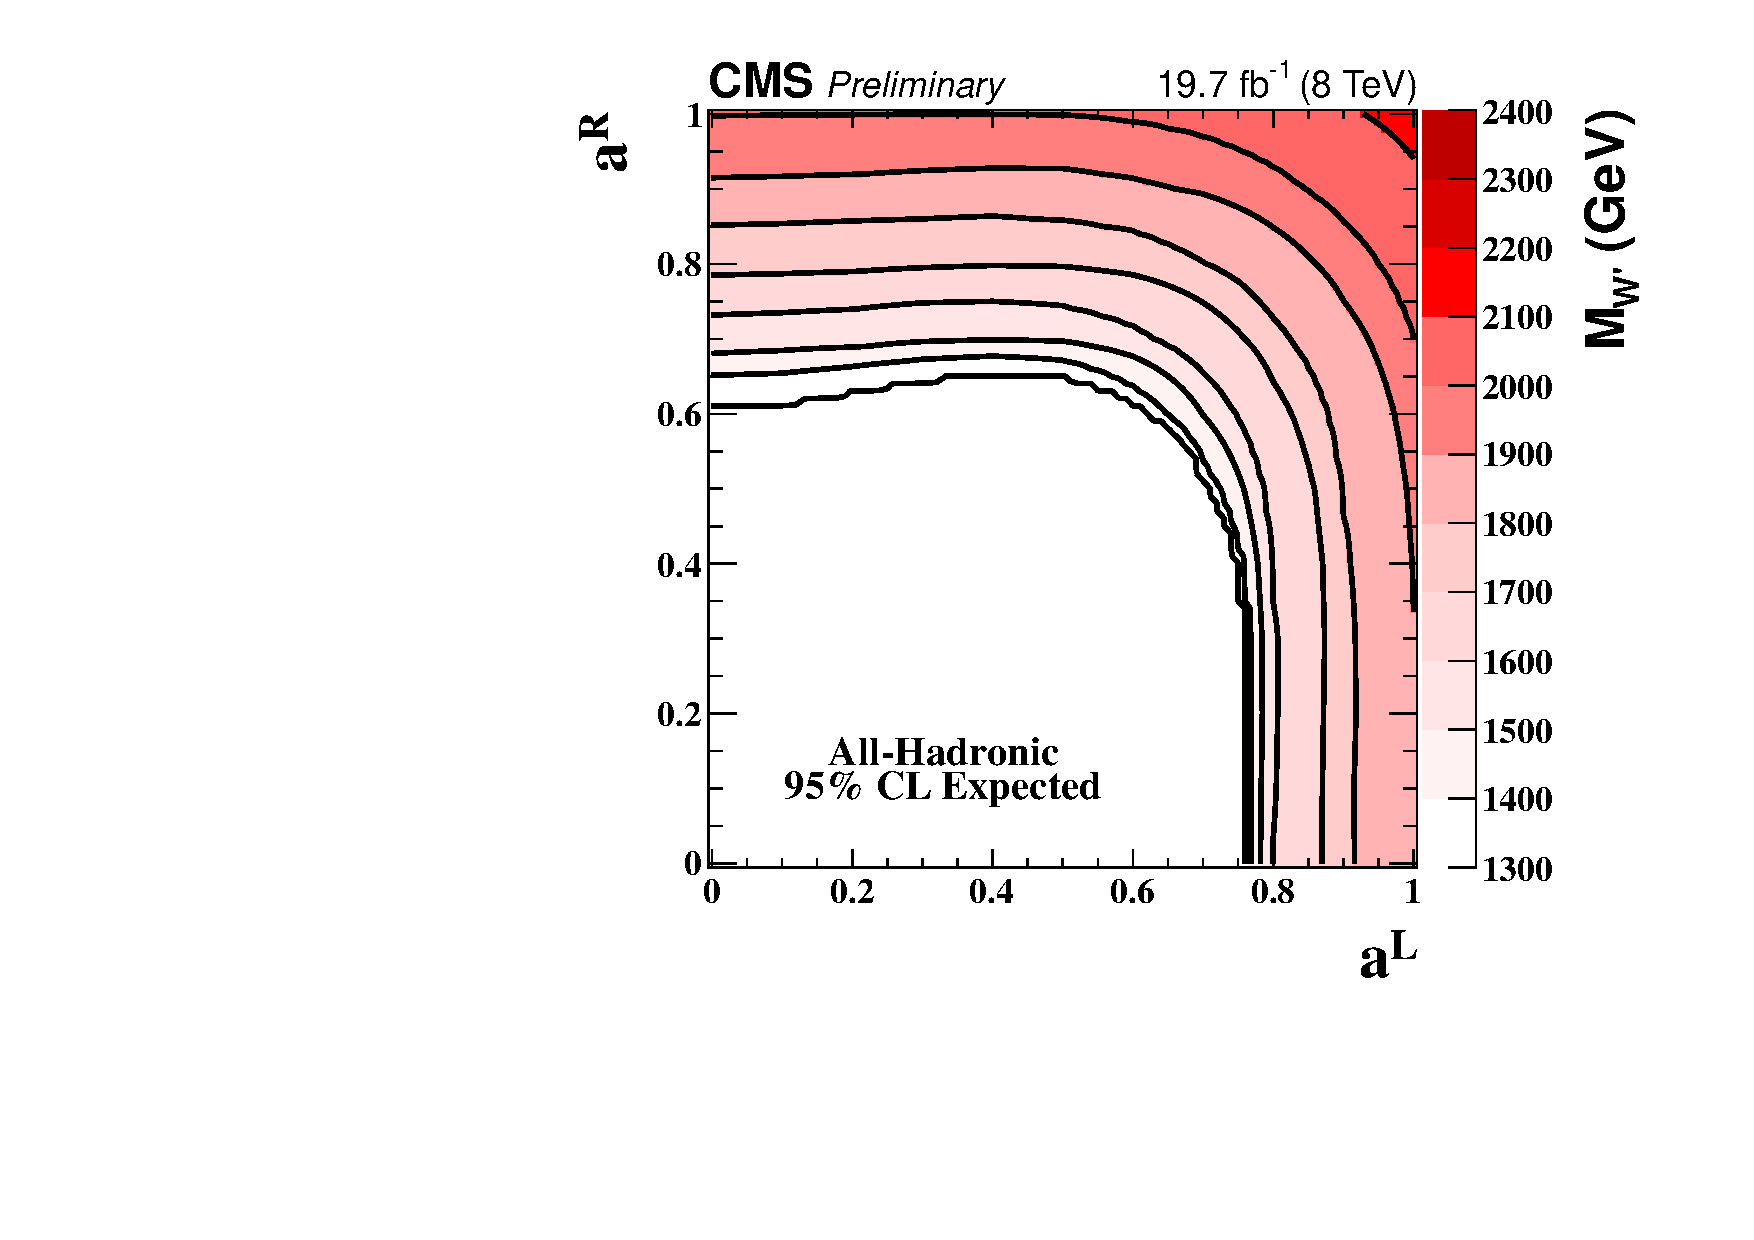
\includegraphics[width=0.7\textwidth]{AN-13-004/figs/contour_Hadronic_expected.pdf}}
\caption{
Plots of $M_{\wpr}$ as a function of $a^L$ and $a^R$.  The z axis colors indicate $M_{\wpr}$ 
where the theoretical cross section intersects the observed or expected limit band.  The top (bottom) plot shows observed (expected) limits.
}
\label{figs:GCLim}
\end{center}
\end{figure}

\begin{figure}[htcb]
\begin{center}
\subfigure{\label{figs:ST1}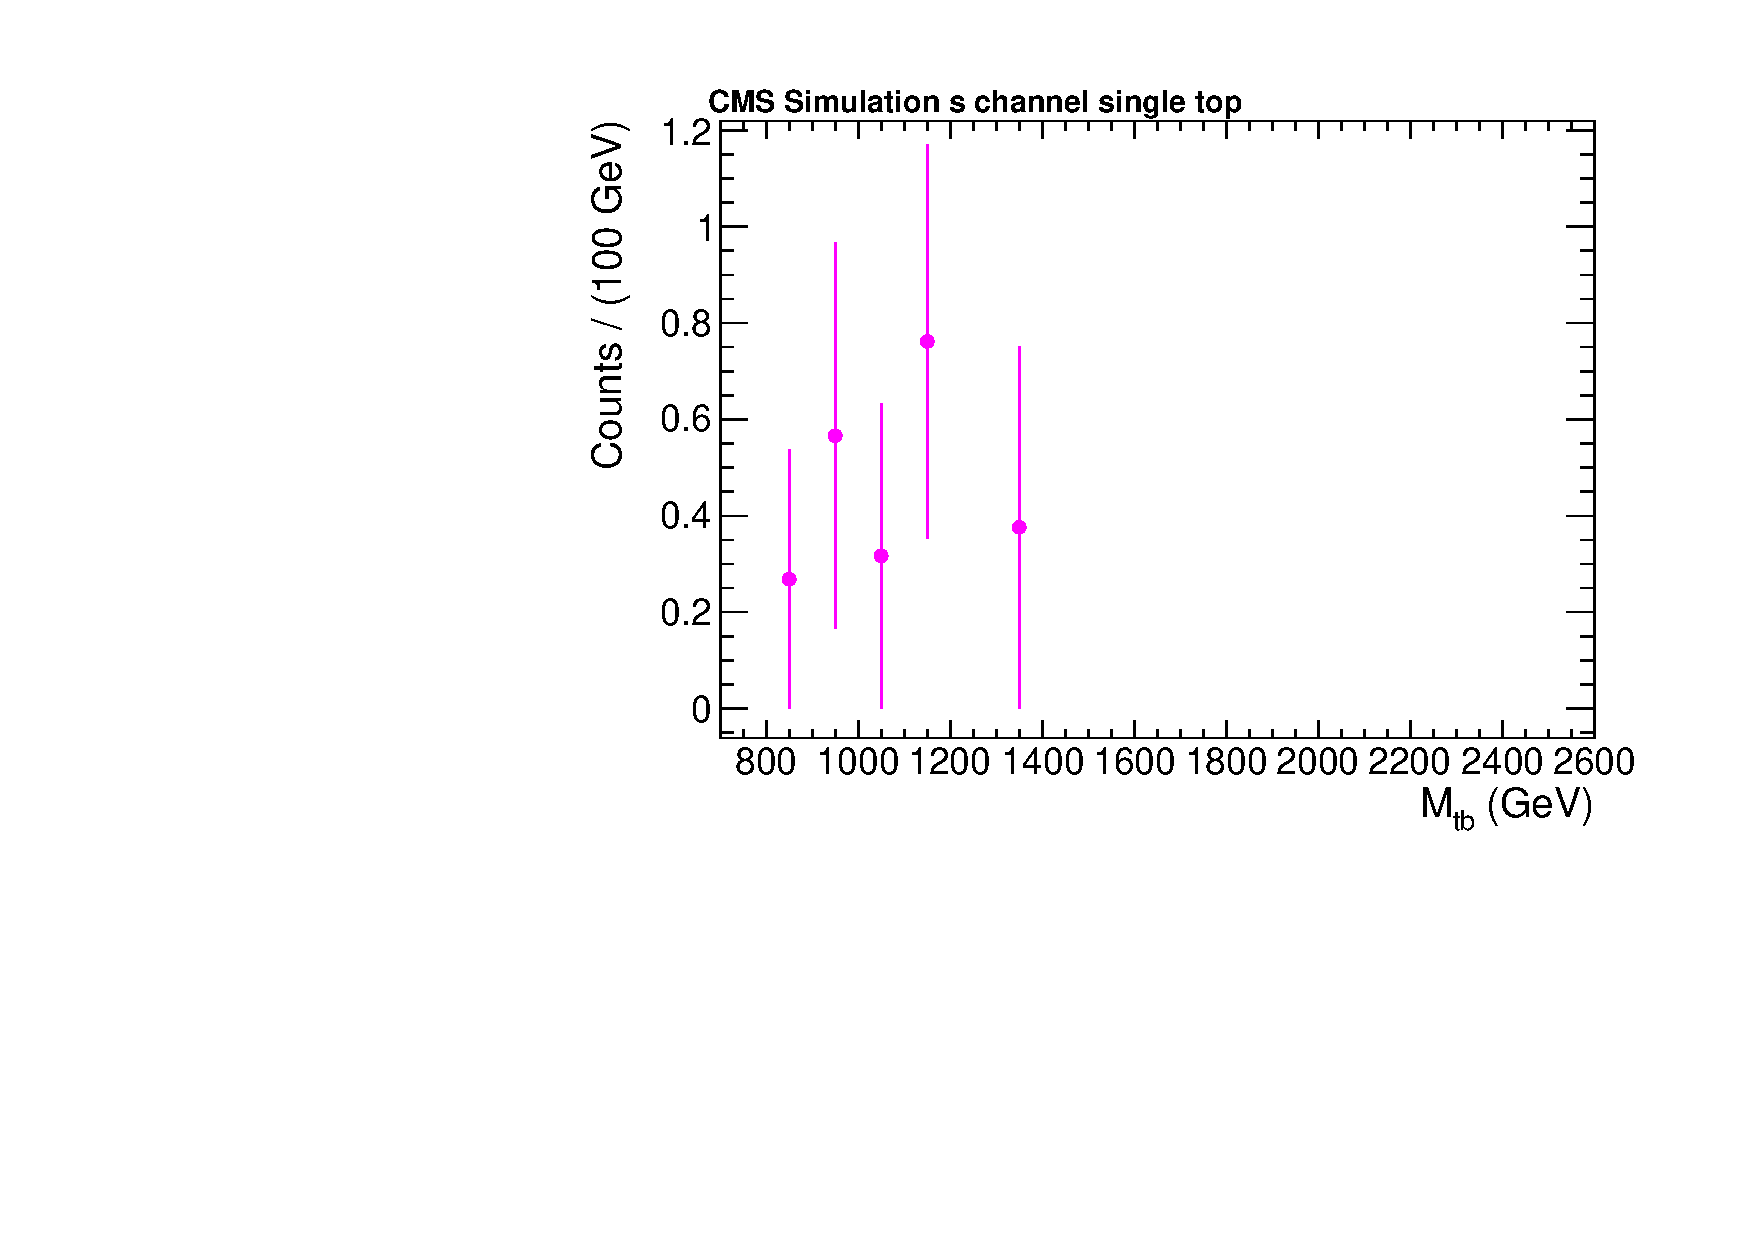
\includegraphics[width=0.7\textwidth]{AN-13-004/figs/schanst.pdf}}
\caption{
Standard model s-channel single top production used for the generalized coupling analysis.
}
\label{figs:ST}
\end{center}
\end{figure}

\clearpage
